\documentclass{article}
\usepackage{graphicx}
\usepackage{listings}
\usepackage{ctex}
\usepackage{graphicx}
\usepackage[a4paper, body={18cm,22cm}]{geometry}
\usepackage{amsmath,amssymb,amstext,wasysym,enumerate,graphicx}
\usepackage{float,abstract,booktabs,indentfirst,amsmath}
\usepackage{array}
\usepackage{booktabs} %调整表格线与上下内容的间隔
\usepackage{multirow}
\usepackage{diagbox}
\usepackage{indentfirst}
\usepackage{bm}
\usepackage{fancyhdr}




\pagestyle{fancy}

\lhead{\bfseries \normalsize 学号:1952033\quad 姓名:侯雅玥 \quad 组员:廖宏 \\实验名称:场效应管放大器\quad 课程名称:电子技术实验\quad 专业:微电子科学与工程 } 
\rhead{}

\begin{document}

	\section{\zihao{4} 实验名称:负反馈放大电路的研究}
    \section{\zihao{4} 实验目的}
    \zihao {5} (1)研究负反馈对放大器各项性能指标的影响\par
	           (2)理解电路中引入负反馈的意义和方法\par
               (3)进一步熟悉放大电路中$A_u,f_L,f_H,$及$R_i,R_o$的测量方法\par
			   \section{\zihao{4} 实验原理}
    场效应管是一种有放大作用的器件,有如下特点:\par
   
(1)场效应管是一种电压控制器件,通过栅极电$u_{GS}$来控制漏极电流$i_D$,从场效应管的输出特性上可以看出,各条不同输出特性曲线的参数变量是$u_{GS}$,在恒流区,$i_D$的值主要取决于$u_{GS}$,而基本与$u_{DS}$无关,如图1所示,并通过跨导$g_m=\frac{\Delta  i_D}{\Delta  u_{GS}}{\bigg |}_{u_{DS}=constant}$来描述场效应管的放大作用。\par
(2)场效应管的栅极几乎不取电流,所以其输入电阻非常高,结型场效应管一般在$10^7$以上\par
(3)场效应管用一种极性的多数载流子导电,因此具有噪音小,受外界温度辐射影响小
  \begin{figure}[h]
	\centering
	  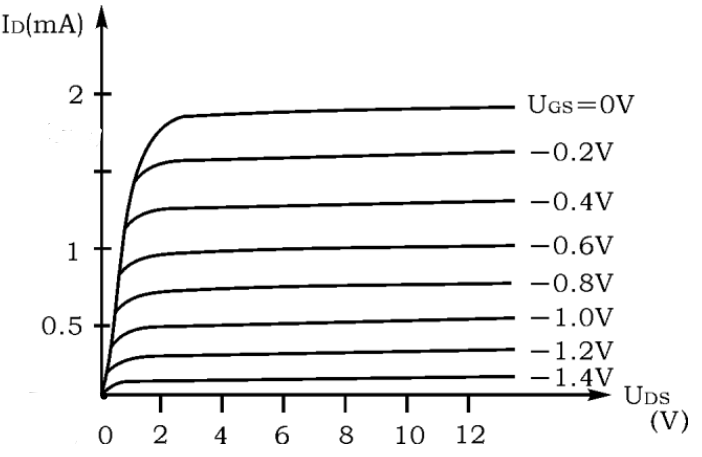
\includegraphics[width=10cm]{H:/电子技术试验/4-6/4-6-0.png}
	\caption{Figure example 1} 
  \end{figure}
	%\small
	

\section{\zihao{4} 实验电路}
基于场效应管的特点,得到如下共栅极放大电路:\par
\begin{figure}[h]
	%\small
	\centering
	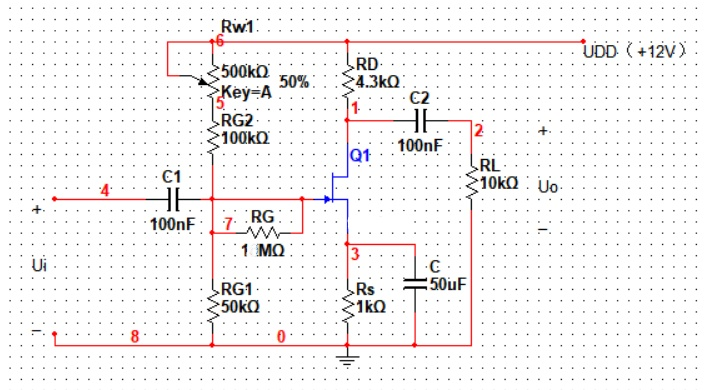
\includegraphics[width=12cm]{H:/电子技术试验/4-6/4-6-1.jpg}
	\caption{Figure example 2} \label{fig:aa}
\end{figure}
\section{\zihao{4} 实验内容及步骤}
\subsection {静态工作点的测量}
(1)按照图2连接电路,接通电源,在放大器的输入端加$f=1kHz$,$U_i=50mV$的正弦信号,调节Rw1,用示波器观察当负载$R_L=\infty$的情况下,输出电压波形不失真时的最大输出电压波形,此时用万用表测量静态工作点的各电压值  \par
\begin{table}[h]
	\centering  
	\begin{tabular}{c|c|c|c|c|c}
		\hline
	        \multicolumn{3}{c}{测量值} \vline    &  \multicolumn{3}{c}{计算值} \\\hline
		    $U_s$  &  $U_D$    & $U_G$     & $U_{DS}$ & $U_{GS}$    &$I_D$    \\ \hline
		    1.085V &  4.876V   & 1.675V    &3.201V    &0.590V      &  1.668mA\\   \hline
	\end{tabular}
	\caption{静态工作点数据表}\label{SIGN}
	\end{table}
	
\subsection{动态指标的测量}
(1)计算电阻$R_i$与$R_o$的估算值\par

(1)测量$A_u$与$R_o$的值\par
在放大器输入端加$f=1kHz,U_i=50mV$的正弦信号,并用示波器监视输出电压的波形,在输出电压$U_o$没有失真的条件下,用交流毫伏表分别测量电路的空载输出电压$U_{o1}$和有负载输出电压$U_{o2}$
\begin{table}[h]
	\centering  
	\begin{tabular}{c|c|c|c|c}
		\hline
	        $U_i$  &  $U_{o1}(R_L=\infty)$    & $U_{o2}(R_L=10k\Omega)$     & $A_{u1}$ & $A_{u2}$        \\ \hline
		    50mV &  241.79mV   & 175.47mV    &5    &3    \\   \hline
	\end{tabular}
	\caption{场效应管放大器数据表}\label{SIGN}
	\end{table}
(2)$R_i$的测量\par
按图3改接电路,取$R=100k\Omega$,选择输入电压$U_s$,保持$U_s$不变,将开关K掷向“1”(R=0),测出输入电压$U_{o1}$,然后将开关K掷向“2”(R=0),测出输入电压$U_{o2}$.
\begin{figure}[h]
	%\small
	\centering
	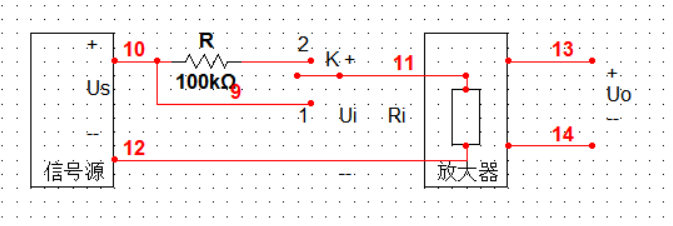
\includegraphics[width=12cm]{H:/电子技术试验/4-6/4-6-2.png}
	\caption{Figure example 3} \label{fig:aa}
\end{figure}
\begin{table}[h]
	\centering  
	\begin{tabular}{c|c|c|c}
		\hline
	        \multicolumn{3}{c}{测量值} \vline    &  \multicolumn{1}{c}{计算值} \\\hline
		    $U_s(mV)$  &  $U_{o1}$    & $U_{o2}$     & $R_i$    \\ \hline
		    50         &  240.67mV   & 218.52mV    &986.55k$\Omega$    \\   \hline
			80         &  441.87mV   & 401.83mV    &1003.57k$\Omega$     \\   \hline
	\end{tabular}
	\caption{测量$R_i$数据表}\label{SIGN}
	\end{table}
	\section{\zihao{4} 数据处理}
	(1)计算电阻$R_i$与$R_o$与$A_u$的估算值
	\begin{equation*}
		\ R_{i0}=R_G+(R_{G1}\|R_{G2})=1033k\Omega\\
		\ R_{o0}=R_D=4.3k\Omega\\
		\ g_m=\frac{2I_D}{V_ov}=0.88\\
		\ A_{u10}=g_m\times R_D=3.8\\
		\ A_{u20}=g_m\times R_D=2.6\\
	\end{equation*}
	(2)计算电压放大器的倍数
	\begin{equation*}
		\ A_{u1}=\frac{U_{o1}}{U_i}=4.8\\
		\ A_{u2}=\frac{U_{o2}}{U_i}=3.5
	\end{equation*}
	填入表格2
	(3)计算输出电阻
	\begin{equation*}
	     \ R_o=\bigg (\frac{U_{o1}}{U_{o2}}-1\bigg )R_L=3.7k\Omega
	\end{equation*}
	(4)$R_i$的计算
	由于,
	\begin{equation*}
		\ U_{o2}=A_u\times U_i=A_u\times\frac{R_i}{R_i+R}\times U_s\\
	\end{equation*}
	由此求得,
	\begin{equation*}
		\ R_i=\frac{U_{o2}}{U_{o1}-U_{o2}}\times R\\
	\end{equation*}
	填入表格3
	\section{\zihao{4} 实验设备和器材}
	(1)双踪示波器             \qquad \qquad \qquad \qquad \qquad  \qquad           1台\par
	(2)函数信号发生器          \qquad  \qquad \qquad \qquad       \qquad           1台\par
	(3)直流稳压电源             \qquad \quad \qquad \qquad \qquad \qquad           1台\par
	(4)模拟电路实验箱            \qquad  \qquad \qquad \qquad\qquad                1台\par
	(5)万用表                   \qquad  \qquad \qquad \qquad \qquad \qquad \qquad  1只\par
	(6)场效应管3DJ6F、电阻器、电容器  \qquad                                        若干
\section{误差处理}

\begin{align*}
	\ \delta (R_i)&=\frac{\overline{R_i}-R_{i0}}{R_{i0}} \times 100\%=3.6\%\\
	\ \delta (R_o)&=\frac{{R_o}-R_{o0}}{R_{o0}} \times 100\%=13.9\%\\
	\ \delta (A_{u1})&=\frac{{A_{u1}}-A_{u10}}{A_{u10}} \times 100\%=22.9\%\\
	\ \delta (A_{u2})&=\frac{{A_{u2}}-A_{u20}}{A_{u20}} \times 100\%=25.7\%\\
\end{align*}    \par
(1)误差可能是器件老化造成。\par
(2)场效应管存在沟道长度调制效应,可能出现测量不精准。
(3)偏置点不一定完全准确
\section{结论}
(1)综上所述,得到静态工作点为$U_{DS}$约为4.9V时,处于静态工作点。\par
(2)$R_o$约为3.7k$\Omega$ ,$R_i$约为995.06k$\Omega$

\section{思考题}
在测量场效应管放大电路静态工作电压$U_{GS}$时,能否用万用表直接在G、S两端测量,为什么?试比较$U_{GS}$直接测量值和间接测量值的差异。\par
在测量场效应管静态工作电压$U_{GS}$时,不能使用万用表直接并在G,S两端测量。因为场效应管各个极阻抗高、受到电磁感应的影响很大,万用表会影响工作点的较大变化,通过万用表直接测量$U_{GS}$得到$U_{GS}=0.225V$误差较大。



\end{document}

